\documentclass[11pt,a4paper]{report}

\usepackage[utf8]{inputenc}
\usepackage[portuges]{babel}
\usepackage{indentfirst}
\usepackage{graphicx}
\usepackage{float}
\usepackage{caption}
\usepackage{subcaption}
\usepackage[T1]{fontenc}
\usepackage{listings}
\usepackage{amsmath}
\usepackage{mathtools}
\usepackage{tikz}
\renewcommand{\familydefault}{\sfdefault}

% packages que adicionei do stor
\usepackage{xspace}
\setlength{\oddsidemargin}{-1cm}
\setlength{\textwidth}{18cm}
\setlength{\headsep}{-1cm}
\setlength{\textheight}{23cm}

\title{Processamento de Linguagens (3º ano de Curso)\\
	\textbf{Trabalho Prático Nº2 (GAWK)}\\ Relatório de Desenvolvimento}
\author{Diogo Braga\\ A82547 \and João Silva\\ A82005 \and Ricardo Caçador\\ A81064}
\date{\today}

\begin{document}

\maketitle

\begin{abstract}
	Neste relatório é apresentada a resolução de um exercício referente ao TP2, que tem como principais objetivos:
	\begin{itemize}
		\item aumentar a experiência de uso do ambiente Linux e de algumas ferramentas de apoio à programação;
 		\item aumentar a capacidade de escrever \textbf{Expressões Regulares} para descrição de \textit{padrões de frases};
 		\item desenvolver, a partir de ERs, sistemática e automaticamente \textit{Processadores de Linguagens Regulares}, que filtrem ou transformem textos;
 		\item utilizar o sistema de produção para filtragem de texto \textbf{GAWK}.
	\end{itemize}
\end{abstract}

\tableofcontents

\newpage

\chapter{Introdução}
\label{chap:intro}

Seguindo a fórmula \emph{exercício = (N\_Alu\% 5)  +  1} e o número de aluno mais baixo presente no nosso grupo (81064), o enunciado correspondente é o \textbf{5 - Processador de textos preanotados com Freeling}.

Este enunciado apresentou-nos um tipo de ficheiro (\textbf{CORPORA}) que agrupam grandes quantidade de textos aos quais adicionam informação de anotação frásica e morfossintática. Estes ficheiros vêm ainda incorporados com o formato \textbf{Freeling} que separa extratos com uma linha em branco, e separa colunas por espaços para a informação morfossintática de cada palavra.

Ao longo deste trabalho produzimos principalmente 4 filtros em \textbf{AWK}, cada um com um objetivo bem delimitado. O primeiro visa contar o número de extratos contidos num determinado ficheiro. O segundo calcula uma lista de personagens de \textit{Harry Potter}, bem como o número de ocorrências associado a cada uma. O terceiro calcula uma lista de verbos,  substantivos, adjectivos e advérbios e mostra o resultado num ficheiro \textbf{HTML}. Por último o quarto filtro tem como objetivo determinar o dicionário implícito \textbf{CORPORA} que é uma lista contendo os lema, pos e palavras dele derivadas.

Com este relatório pretendemos apresentar as nossas opções, algoritmos desenvolvidos e ainda estruturas utilizadas para a realização de cada filtro. Pretendemos também apoiar aquelas que foram as nossas soluções, com conhecimento obtido nas aulas teóricas.

Para uma melhor visão do que irá ser abordado neste relatório deixamos uma breve descrição daquilo que foi feito. No segundo capítulo foi feita uma análise informal e uma especificação dos requisitos deste projeto. No terceiro capítulo foi realizado o desenho da conceção no qual estão envolvidos os algoritmos e estruturas de dados usados. No quarto capítulo mostramos alguns exemplos de implementações e vários resultados de testes realizados. Por último no capítulo 5 fazemos uma retrospetiva do trabalho realizado e concluímos.



\chapter{Análise e Especificação}
\label{chap:analise}

Analisando o problema como um todo o que podemos encontrar aquando da observação dos ficheiros \textbf{fl0}, \textbf{fl1}, \textbf{fl2}, \textbf{harrypotter1} e \textbf{harrypotter2}, é a apresentação de vários extratos com detalhes relacionados com a anotação frásica e morfossintática de cada palavra. O nosso objetivo principal é filtrar o que achamos necessário para cumprir os requisitos impostos pelo enunciado e descritos nas subsecções seguintes.

Nas secções seguintes serão apresentados os objetivos de cada alínea do exercício e ainda as observações que foram feitas ao ficheiro, por forma a pensar que casos iríamos ter futuramente e começarmos a delinear uma arquitetura duma possível solução.

\section{Análise e Especificação dos Requisitos}
\subsection{Número de Extratos}
\label{subsec:analise1}

Na primeira alínea do exercício, era requerido um filtro que contasse o número de extratos de um ficheiro CORPORA Freeling.

Ao proceder à análise dos ficheiros concluímos que, como já tinha sido projetado no enunciado, o formato Freeling separa extratos com uma linha em branco.

É importante referir que, no caso destes ficheiros, a pontuação nos extratos é contabilizada como sendo palavras.

\vspace{0.5cm}

Na figura \ref{img:analise1} é possivel verificar:

\begin{enumerate}
 \item Fim de um extrato de 10 palavras finalizada com '.';
 \item Espaço que indica mudança de extrato;
 \item Extrato "O senhor Dursley ficou transido.", com 6 palavras;
 \item Espaço que indica mudança de extrato;
 \item Extrato "O medo apoderou se de ele.", com 7 palavras;
 \item Espaço que indica mudança de extrato;
 \item Início de um extrato iniciado com "Olhou para".
\end{enumerate}

\begin{figure}[H]
\centering
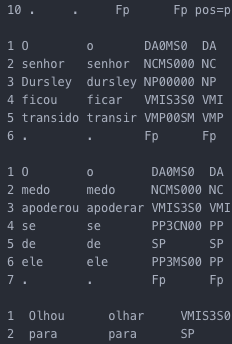
\includegraphics[scale=0.6]{analise1.png}
\caption{Exemplo de dois extratos no ficheiro harrypotter1.}
\label{img:analise1}
\end{figure}

\subsection{Personagens do Harry Potter}
\label{subsec:analise2}

Na alínea b, foi pedido uma listagem das personagens do Harry Potter e as suas respetivas ocorrências. Depois de uma primeira análise ao ficheiro percebeu-se que todas as personagens do Harry Potter na 7ª coluna dos documentos a analisar conteriam grup-nom-ms:[0-9] e w-ms:[0-9], significando que seriam nomes próprios. Assim não havendo uma forma de distinguir um nome próprio de uma localidade com o nome próprio de uma personagem, o nosso filtro baseou-se então nessa abordagem.

\begin{figure}[H]
\centering
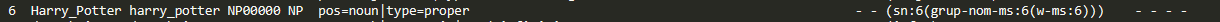
\includegraphics[scale=0.7]{harry1.png}
\caption{Exemplo uma personagem do Harry Potter no ficheiro a ser analisado}
\label{img:harry1}
\end{figure}

\subsection{Palavras por Classes em HTML}

A terceira alínea do exercício requeria que fosse criado um filtro capaz de calcular uma lista de verbos, substantivos, adjectivos e advérbios. Consequentemente deveria ser colocado num ficheiro HTML cada uma destas listas.

Numa primeira abordagem ao problema foram analisadas as possíveis formas de apresentação de cada classe de palavras a serem filtradas.

Atendendo ao formato Freeling dum ficheiro CORPORA, foram de fácil verificação os seguintes factos, relativos à 6ª coluna de cada extrato:

\begin{enumerate}
 \item Se uma palavra for um verbo, então "pos=verb" está contido neste campo;
 \item Se uma palavra for um substantivo, então "pos=noun" está contido neste campo;
 \item Se uma palavra for um adjetivo, então "pos=adjective" está contido neste campo;
 \item Se uma palavra for um advérbio, então "pos=adverb" está contido neste campo;
\end{enumerate}

Foram ainda necessárias criar algumas bases na linguagem de programação HTML relativas à estruturação dum ficheiro, à criação dum cabeçalho e à listagens de elementos. Estas foram basicamente todas as operações necessárias, usadas nesta linguagem, para a realização desta alínea.


\subsection{Dicionário}
\label{subsec:analise4}

Nesta quarta alínea do exercício era requerida a apresentação de um dicionário implícito num ficheiro corpora. Este dicionário deve conter as lemas, as palavras derivadas das lemas, e a informação relativa a essas mesmas palavras. Esta informação vem dividida em colunas.

Realizando a análise de cada ficheiro concluímos que, para a resolução deste exercício o que nos interessava era:

\begin{itemize}
 \item Segunda coluna $\Rightarrow$ Palavra
 \item Terceira coluna $\Rightarrow$ Lema da Palavra
 \item Sexta coluna $\Rightarrow$ Informação da Palavra
\end{itemize}

\vspace{0.5cm}

Na figura \ref{img:analise4} é possivel verificar:

\begin{enumerate}
	\item Palavra $\Rightarrow$ Dumbledore ; Lema $\Rightarrow$ dumbledore ; Informação $\Rightarrow$ Noun Proper ;
	\item Palavra $\Rightarrow$ voltou ; Lema $\Rightarrow$ voltar ; Informação $\Rightarrow$ Verb Main Indicative Past 3 Singular ;
	\item Palavra $\Rightarrow$ se ; Lema $\Rightarrow$ se ; Informação $\Rightarrow$ Pronoun Personal 3 Common Invariable ;
	\item Palavra $\Rightarrow$ e ; Lema $\Rightarrow$ e ; Informação $\Rightarrow$ Conjunction Coordinating ;
	\item Palavra $\Rightarrow$ desceu ; Lema $\Rightarrow$ descer ; Informação $\Rightarrow$ Verb Main Indicative Past 3 Singular ;
	\item Palavra $\Rightarrow$ a ; Lema $\Rightarrow$ o ; Informação $\Rightarrow$ Determiner Article Feminine Singular ;
	\item Palavra $\Rightarrow$ rua ; Lema $\Rightarrow$ rua ; Informação $\Rightarrow$ Noun Common Feminine Singular ;
	\item Palavra $\Rightarrow$ . ; Lema $\Rightarrow$ . ; Informação $\Rightarrow$ Punctuation Period ;
\end{enumerate}


\begin{figure}[H]
\centering
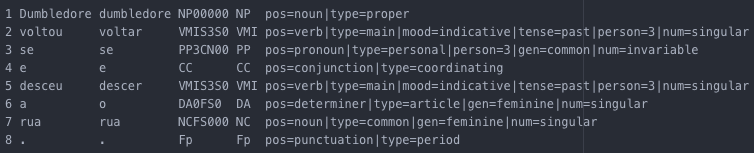
\includegraphics[scale=0.6]{analise4.png}
\caption{Exemplo de um extrato no ficheiro harrypotter1.}
\label{img:analise4}
\end{figure}


\chapter{Conceção/desenho da Resolução}
\label{chap:concecao}

Neste capítulo baseamo-nos nas análises feitas aos ficheiros que serviram de input ao filtros, e construímos os algoritmos para a resolução de cada alínea requisitada no enunciado.

\section{Algoritmos}
\subsection{Número de Extratos}
\label{subsec:algoritmos1}

Para este filtro, os valores associados ao \textbf{Register Separator} e ao \textbf{Field Separator} mantiveram-se os pré-definidos.

Tendo em conta a secção \ref{subsec:analise1}, no qual foi concluído que os extratos eram separados por uma linha em branco, é também característica dum ficheiro CORPORA Freeling o facto dos extratos conterem as posições das suas palavras.

Desta forma, a implementação deste filtro passa por utilizador um contador, inicializado a 0 no bloco \textbf{BEGIN}, que é incrementado cada vez que a primeira coluna duma linha é \textbf{"1"} (string).

Esta abordagem faz sentido pois, para estarmos perante um extrato, este tem que ser inicializado com uma primeira palavra, e desta forma, estamos a contabilizar o número de vezes que um extrato é inicializado. Ou seja, estamos a contabilizar o número de extratos que existem.

No final, no bloco de \textbf{END}, é impresso o contador que contêm o número de extratos presentes no ficheiro.


\subsection{Personagens do Harry Potter}
\label{sub:algoritmos2}

Neste filtro para as personagens do Harry Potter o método de resolução passou então pela filtragem de todos os nomes que contivessem os campos referidos na secção 2. Para isso foi utilizado um array associativo que em cada índice incrementaria a ocorrência de uma personagem. Assim, tornou-se fácil a apresentação das respetivas ocorrências de cada personagem através da impressão desse mesmo array no terminal.
Esta abordagem vai apanhar algum "lixo", ou seja, nomes próprios que não sejam personagens do Harry Potter mas foi a única abordagem que o grupo conseguiu desenvolver que apanhasse realmente todas as personagens da história.


\newpage

\subsection{Palavras por Classes em HTML}
\label{sub:algoritmos3}

Inicialmente no bloco de \textbf{BEGIN} não alteramos nada que fosse relativo ao \textbf{Register Separator}, nem ao \textbf{Field Separator}, pelo que os valores associados a estes campos se mantiveram os pré-definidos. Neste bloco é realizada a criação duma pasta \textbf{C\_HTML} que albergará todos os ficheiros HTML necessários, e ainda é criado o ficheiro \textit{index.html} que corresponde ao ficheiro que é um índice de redirecionamento para outros.

Consoante a análise realizada no capítulo anterior, a parte do uso de expressões regulares para a filtragem das classes de palavras ficou facilitada uma vez que foi preciso apenas descriminar cada caso existente, todos eles relacionado com o 6º campo de cada registo. As expressões utilizadas foram as seguintes:

\begin{itemize}
	\item \$6 $\sim$ /pos=verb/
	\item \$6 $\sim$ /pos=adjective/
	\item \$6 $\sim$ /pos=adverb/
	\item \$6 $\sim$ /pos=noun/
\end{itemize}

Consoante cada classe, cada palavra filtrada era inserida num array associativo correspondente.

Finalmente no bloco de \textbf{END} é tratada a maior parte da construção de ficheiros HTML, e inserido nestes tudo o que foi filtrado. Criámos então 3 funções em AWK para se responsabilizarem desta tarefa. Estas são:

\begin{itemize}
	\item make\_page\_html(arg)
	\begin{itemize}
		\item Esta função é responsável pela criação dum ficheiro, cujo nome é passado como parâmetro (arg), e do seu cabeçalho.
	\end{itemize}
	\item list\_elem\_html(elem,filename)
	\begin{itemize}
		\item Esta função é responsável por adicionar ao ficheiro, cujo nome é passado como parâmetro (filename), um elemento a ser listado, também passado em argumento (elem).
	\end{itemize}
	\item make\_end\_html(arg)
	\begin{itemize}
		\item Esta função é responsável por terminar o ficheiro, cujo nome é passado como parâmetro (arg).
	\end{itemize}
\end{itemize}

As funções \textbf{make\_page\_html(arg)} e \textbf{make\_end\_html(arg)} são usadas somente uma vez. Entre elas é realizado um ciclo que percorre o array associativo correspondente, e ao ficheiro respetivo é adicionado o elemento que reside no array através da função \textbf{list\_elem\_html(elem,filename)}

\newpage

\subsection{Dicionário}
\label{subsec:algoritmos4}

No bloco de \textbf{BEGIN}, como o \textbf{Register Separator} e o \textbf{Field Separator} são os pré-definidos, nada foi alterado. Neste bloco é realizada apenas a impressão duma string a indicar que iriamos estar perante um dicionário.

Tendo em conta a análise realizada na secção \ref{subsec:analise4}, para a conceção desta solução são necessárias a segunda, a terceira, e a sexta coluna, respetivamente, as palavras , as lemas associadas às palavras, e a informação das palavras.

O corpo principal deste filtro divide-se em 3 fases:

\begin{enumerate}
	\item Associação da informação da palavra à palavra em questão:
		\begin{itemize}
			\item Palavra $\Rightarrow$ \$2
			\item Informação da palavra $\Rightarrow$ \$6
			\item Função \textbf{posGenSub} que torna mais perceptível a informação da palavra utilizando a função pré-definida em AWK \textbf{gsub};
			\item Função \textbf{gsub} que substitui "|" por "\hspace{0.12cm} : ", de forma à informação ficar, portanto, mais separada;
			\item Criação duma string \textbf{palPos} que vai concatenar o \$2 com o resultado da função \textbf{posGenSub};
		\end{itemize}
	\item Associação das palavras à lema que as define:
		\begin{itemize}
			\item Lema $\Rightarrow$ \$3
			\item Utilização dum array associativo \textbf{palavras} no qual o indíce é a lema;
			\item Função \textbf{palavrasFunc} que concatena as palavras que possuem a mesma lema, com auxílio da função pré-definida em AWK \textbf{index};
			\item Função \textbf{index} que verifica se a palavra e sua informação respetiva ainda não estão associadas à lema em questão, verificando se a palavra e respetiva informação já estão presentes na string da posição do array associativo em que o índice é a lema;
			\item Caso não esteja presente, ou seja, caso a função \textbf{index} retorne 0, é concatenada a nova palavra e sua respetiva informação com o que já estava definido;
		\end{itemize}
	\item Criação duma string que vai concatenar a lema com as palavras derivadas:
		\begin{itemize}
			\item Utilização dum array associativo \textbf{res} no qual o indíce é a lema;
			\item Valor de cada índice é a string que junta a lema \$3 com o valor do array associativo \textbf{palavras} no qual o índice é \$3;
		\end{itemize}
\end{enumerate}

No bloco \textbf{END} é utilizada a função pré-definida em AWK \textbf{asort}, que organiza os valores do array associativo \textbf{res} crescentemente. Desta forma, como a lema é a primeira parte das strings do array associativo, o dicionário vai ficar definido por ordem alfabética.

Ainda neste bloco final, é impresso todo o array associativo \textbf{res}, originando assim um dicionário do ficheiro passado como parâmetro ao AWK.


\chapter{Codificação e Testes}
\label{chap:codificacao}

Para a presente secção de codificação e testes baseámo-nos nos capítulos anteriores, pois ambos são extremamente importantes para uma boa implementação desta fase. O capítulo de análise teve a sua relevância pois permitiu-nos ter já uma ideia de que expressões regulares utilizar para filtrar o que desejávamos e o capítulo da conceção da resolução foi relevante pois definimos os algoritmos necessários para coordenar o processo de filtragem para cada requisito.

\section{Estruturas de Dados}

\subsection{Personagens do Harry Potter}

Nesta alínea utilizamos os  \textbf{arrays associativos} já implementada em \textbf{AWK} de forma a mapear todas as personagens e incrementar as suas ocorrências.

\begin{figure}[H]
\centering
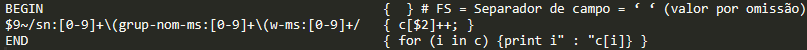
\includegraphics[scale=0.9]{harry.png}
\caption{Codificação do filtro}
\label{img:harry}
\end{figure}



\subsection{Palavras por classes em HTML}

Na terceira alínea foi necessário utilizar fundamentalmente uma estrutura de dados que já vem implementada em \textbf{AWK}, que são os \textbf{arrays associativos}. Foram de imensa utilidade uma vez que mapeiam todos os elementos necessários sem os repetirem.

Para esta alínea utilizamos 4 arrays deste género cada um para cada classe de palavras (verbos, substantivos, adjetivos e advérbios).

\subsection{Dicionário}

Nesta alínea foi necessário utilizar 2 \textbf{arrays associativos}:

\begin{itemize}
	\item \textbf{palavras}
		\begin{itemize}
			\item Relaciona as palavras à lema que as define;
		\end{itemize}
	\item \textbf{res}
		\begin{itemize}
			\item Concatena a lema com as palavras derivadas;
		\end{itemize}
\end{itemize}

\section{Alternativas, Decisões e Problemas de Implementação}

\subsection{Número de Extratos}

Além da solução apresentada na secção \ref{subsec:algoritmos1}, foi identificada outra forma de proceder à resolução desta alínea. A solução dessa secção tinha como principal ideia contar o início dos excertos.

Por outro lado, e tendo em conta que uma linha em branco marca o final de um excerto, a solução podia passar também por contabilizar as linhas em branco.

Para atingir essa solução apenas seria necessário alterar a condição que incrementa o contador para: \underline{$\$1==``"$}

Desta forma, iriamos contabilizar as linhas no qual o primeiro campo não teria nenhuma informação, ou seja, as linhas em branco.

\subsection{Personagens do Harry Potter}

Antes de chegarmos à solução final que foi apresentada, o grupo optou por tentar fazer uma expressão regular para cada uma das personagens que aparecesse na história porém optamos por não continuar com essa solução pois sentimos que não estávamos a aproveitar de todo a capacidade do AWK e seria díficil apanhar todas as personagens, principalmente as que tivessem poucas ocorrências.


\subsection{Dicionário}

Além da solução apresentada na secção \ref{subsec:algoritmos4}, foi identificada outra forma de proceder à resolução desta alínea.

Esta nova solução passava por ter em conta as tags da informação das palavras, que residem na coluna \$5, ao invês da informação mais detalhada que reside na coluna \$6.

A partir das tags, existia uma função que fazia a tradução para a especificação da informação da palavra. Por exemplo, a tag \textbf{VMI} retornava \textbf{"VMI: Verb Main Indicative"}, e seria esta a informação associada à palavra ao invês da que foi apresentada na secção \ref{subsec:algoritmos4}.

Decidimos apresentar como principal solução a resolução anterior porque essa é, de facto, mais detalhada, e achamos que isso seria mais benéfico para o nosso dicionário.


\section{Testes realizados e Resultados}
\subsection{Número de Extratos}

Aplicando o filtro criado para a primeira questão com qualquer um dos ficheiros de input disponibilizados, verificam-se resultados com um formato como o da seguinte imagem.

A informação fornecido é o número de extratos.

\begin{figure}[H]
\centering

\includegraphics[scale=0.7]{testes1.png}
\caption{Resultado do filtro 1 para o ficheiro fl0.}
\label{img:testes1}
\end{figure}

\newpage

\subsection{Personagens do Harry Potter}

Como é visível, este filtro não consegue distinguir os nomes próprios de personganes de outro tipo de nomes próprios, porém, todas as personagens que participem na história são apresentadas no resultado.

\begin{figure}[H]
\centering
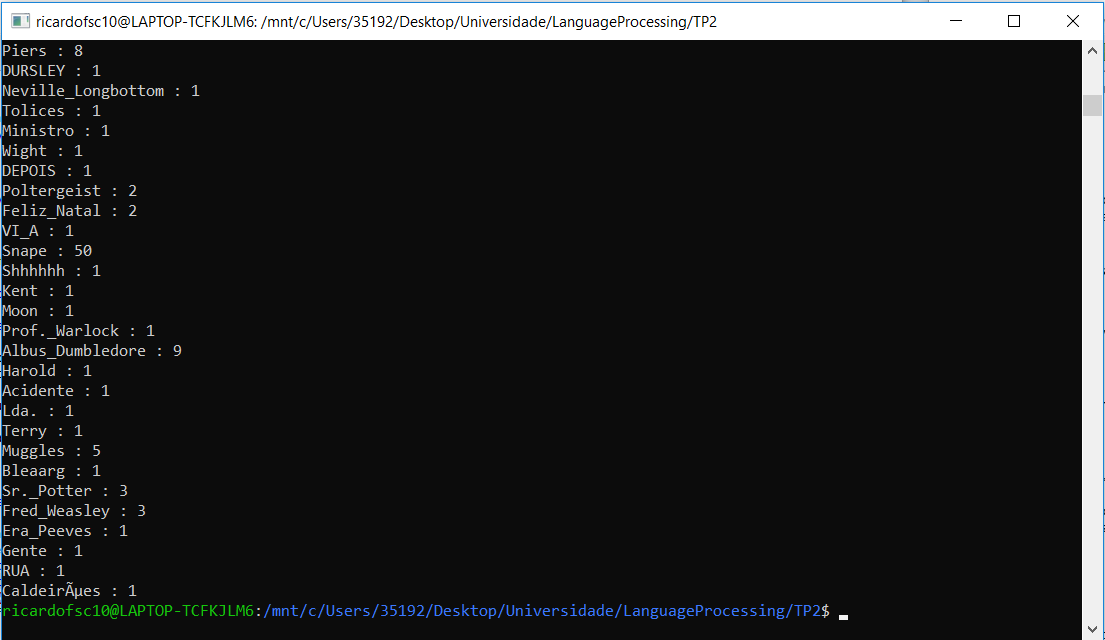
\includegraphics[scale=0.7]{resultadoharry.png}
\caption{Resultado da aplicação do filtro}
\label{img:resultadoharry}
\end{figure}


\subsection{Palavras por Classes em HTML}

O resultado do filtro criado e executado com algum dos ficheiros de input é a criação duma pasta \textbf{C\_HTML} que contém 5 ficheiros HTML. Um destes ficheiros funciona como um índice (\textbf{index.html}) que redireciona para outras páginas HTML. Todos os restantes ficheiros contêm uma lista, ou de verbos, ou de substantivos, ou de adjetivos, ou ainda de advérbios.

A seguir são apresentadas algumas imagens dos resultados em páginas num browser.

\begin{figure}[H]
\centering
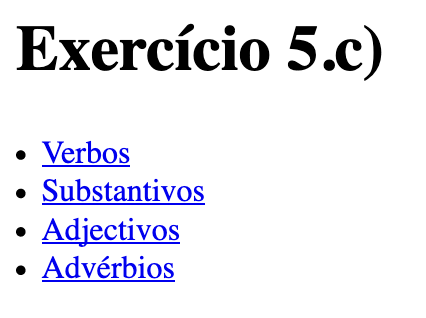
\includegraphics[scale=0.6]{index.png}
\caption{índice criado.}
\label{img:index}
\end{figure}

Carregando em algum dos elementos listados, redireciona-nos para outra página HTML do género das seguintes.

\begin{figure}[H]
\centering
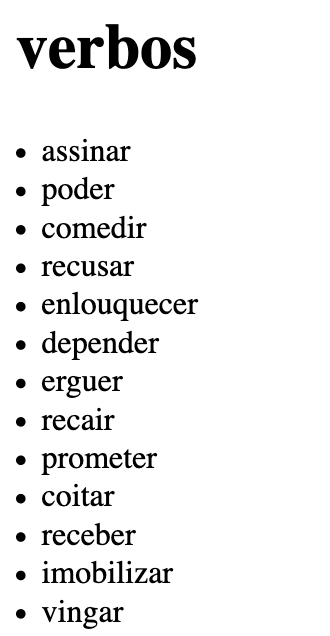
\includegraphics[scale=0.6]{verbos.png}
\caption{Exemplo dum ficheiro com uma lista de verbos.}
\label{img:verbos}
\end{figure}

\begin{figure}[H]
\centering
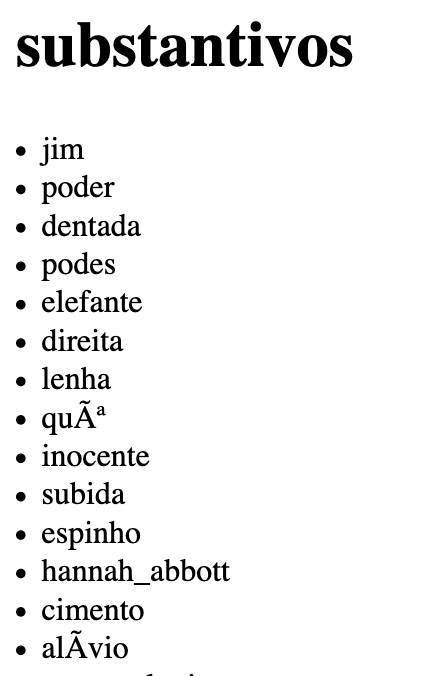
\includegraphics[scale=0.6]{substantivos.png}
\caption{Exemplo dum ficheiro com uma lista de substantivos.}
\label{img:substantivos}
\end{figure}

\begin{figure}[H]
\centering
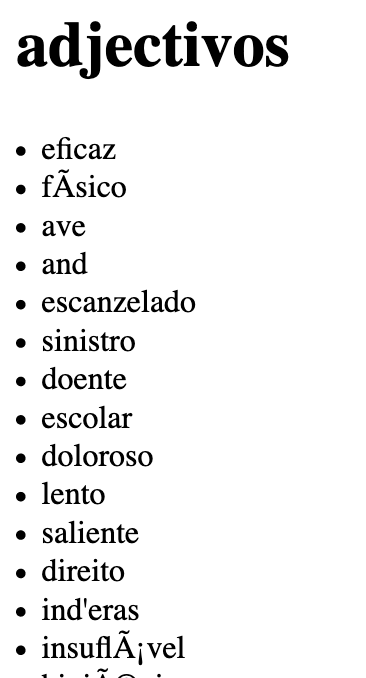
\includegraphics[scale=0.6]{adjetivos.png}
\caption{Exemplo dum ficheiro com uma lista de adjetivos.}
\label{img:adjetivos}
\end{figure}

\begin{figure}[H]
\centering
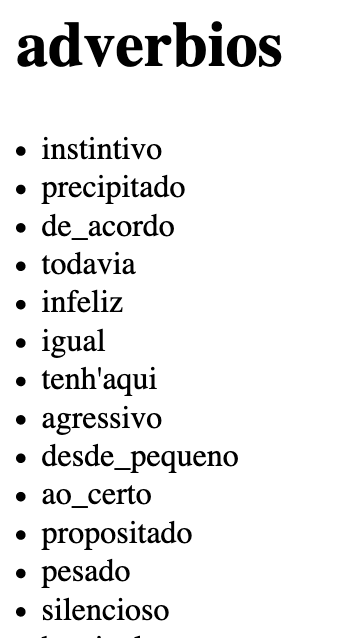
\includegraphics[scale=0.6]{adverbios.png}
\caption{Exemplo dum ficheiro com uma lista de adverbios.}
\label{img:adverbios}
\end{figure}

\newpage

\subsection{Dicionário}

A seguinte imagem apresenta um excerto do resultado do filtro que constrói um dicionário com base num dos ficheiros escolhidos como parâmetro.

O dicionário, conforme pode ser verificado, é apresentado por ordem alfabética, e cada uma das palavras derivadas contêm a sua informação morfossintática.

\begin{figure}[H]
\centering
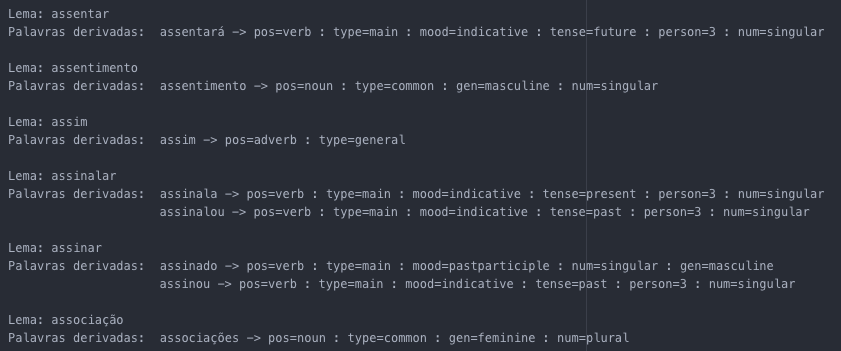
\includegraphics[scale=0.5]{testes4.png}
\caption{Excerto do resultado do filtro 4 para o ficheiro fl1.}
\label{img:testes4}
\end{figure}


\chapter{Extras}
\label{chap:extras}

Como extras ao trabalho realizamos um ficheiro que \textbf{Filtro.awk} que contêm um filtro que engloba todas as alíneas realizadas anteriormente, e o seu resultado é mostrado em HTML.

Realizamos este extra para facilitar a visualização de todos os resultados às questões do enunciado, e porque desta forma é necessário apenas realizar uma filtragem ao ficheiro de input em vez de 4 vezes no caso de testar cada alínea individualmente. Os ficheiros criados em HTML são colocados numa pasta criada no início do filtro que é \textbf{RESULTADOS\_HTML}.

As seguintes imagens representam alguns dos resultado em HTML.

\begin{figure}[H]
\centering
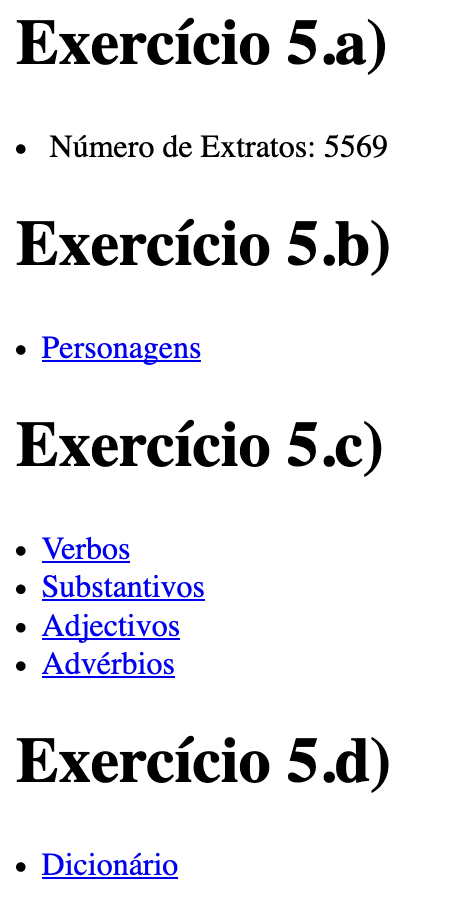
\includegraphics[scale=0.6]{index_resultado.png}
\caption{Índice dos resultados gerados.}
\label{img:indice_resultados}
\end{figure}

\begin{figure}[H]
\centering
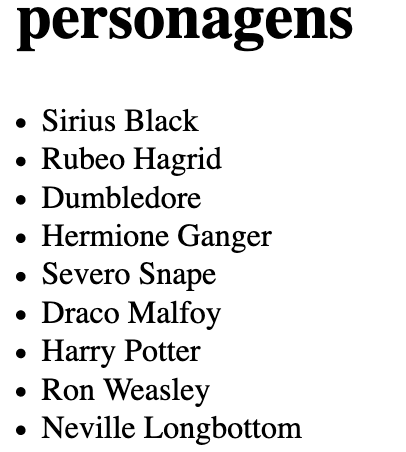
\includegraphics[scale=0.6]{personagens_resultado.png}
\caption{Ficheiro que contém as personagens.}
\label{img:personagens_resultados}
\end{figure}


\chapter{Conclusão}
\label{chap:concl}

Tendo em conta os requisitos deste projeto, e o trabalho realizado pelo grupo, achamos que os objetivos fundamentais foram atingidos, sendo estes a capacidade de criar padrões com uso de \textbf{Expressões Regulares}, o entendimento das capacidades da ferramenta \textbf{AWK} e a capacidade de analisar ficheiros de entrada, assim como a capacidade de criar algoritmos de resolução dos enunciados propostos.

Ao longo da realização deste projeto o grupo procurou saber sempre mais sobre a resolução de cada pergunta, de forma a chegar à melhor resolução possível. É exemplo disso a procura de muitas funções pré-definidas em AWK.

O grupo tentou também apurar ao máximo o espírito crítico, de forma a tomar as melhores decisões nos algoritmos tendo em conta as capacidades da ferramenta AWK, sendo que este foi também um dos maiores desafios encontrados.

Em jeito de conclusão o grupo acha que todas as alíneas requisitadas no enunciado foram terminadas com sucesso, e os objetivos principais deste projeto foram atingidos.

\end{document}
